



\section{RFID}
\todo{Fill section}
%https://en.wikipedia.org/wiki/Radio-frequency_identification
%https://www.ftc.gov/reports/rfid-radio-frequency-identification-applications-implications-consumers-workshop-report
%http://www.rfidjournal.com/articles/view?2481
%http://www.waste360.com/route-optimization/rfid-still-early-stages-adoption-waste-industry
%https://www.dailydot.com/debug/nfl-rfid-player-tracking-zebra-technologies/
%https://web.archive.org/web/20080411211453/http://www.consumergoods.com/ME2/dirmod.asp?sid=&nm=&type=Publishing&mod=Publications%3A%3AArticle&mid=8F3A7027421841978F18BE895F87F791&tier=4&id=07CA1C544D3E4FD1916C7A6D2638913E
%https://www.futuremarketinsights.com/reports/rfid-readers-market

An RFID system in its simplest form consists of a reader, sometimes called an interrogator and a tag. 


\subsection{EM4100}
The EM4100 protocol is widely used for RFID applications on the 125 kHz frequency. So much so that nearly all current readily available RFID passive tags use it. That is if one dont need any security in the application. In fact a EM4100 compatible tag simply has a 64 bit ROM that cointains all the data, so anyone with a compatible reader can read out the data. \cite{EM4100}\\

This also means that once one has programmed the chip, you can not change its ID. The format of the data can be found in figure \ref{fig:03:EM4100_structure}.

\begin{figure}[H]
    \centering
    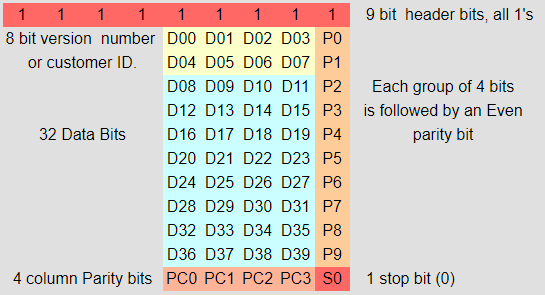
\includegraphics[width=0.8\textwidth]{03_Theory/figures/Datta_layout.png}
    \caption{Data structure of the EM4100 protocol}
    \label{fig:03:EM4100_structure}
\end{figure}

Here we see the start frame of 9 1's, due to the structure of the data, this is the only place we can get more than 9 bits of the same value in a row, due to the even partity bits P1-...-P9 and PC0-...-PC3 and the stop bit S0. The data comes in snippets of 4 bits D00-...-D39 where the first 8 are version number or customer ID. Then following the 32 bit data making up the actual ID.\\

So long as the tag is present in the magnetic field set up by the reader, it will loop through this data over and over. An example of how a tags data may look is shown below.
\begin{figure}[H]
    \centering
    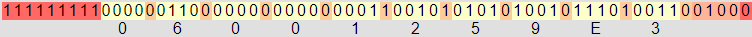
\includegraphics[width=\textwidth]{03_Theory/figures/Dataframe.png}
    \caption{A dataframe from a tag with EM4100}
    \label{fig:03:Dataframe}
\end{figure}

\subsection{Data modulation}

Other than structure of the data, the data needs to have a physical pattern it follows, so as it is possible to detect. This is called data modulation. There is many ways to modulate data, and for a reader to be able to interpret the signal, it is necessary to know its modulation. Three of the more popular modulation schemes are 

\begin{itemize}
    \item Biphase
    \item Phase Shift Key
    \item Manchester
\end{itemize}



\subsubsection{Biphase}
As can be seen in figure \ref{fig:03:biphase} biphase modulation uses the time between the shift from logic high to logic low to determine "1" and "0". To represent a logic high, the signal does not change for one bit length, while for a zero it does. By using  a timer and checking the time since last change, one can determine whether it was a "1" or a "0".

\begin{figure}[H]
    \centering
    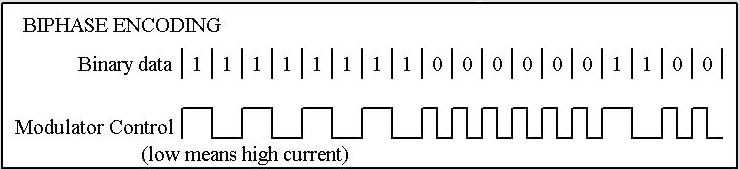
\includegraphics[width=\textwidth]{03_Theory/figures/BIPHASE.png}
    \caption{Biphase encoded RFID tag output}
    \label{fig:03:biphase}
\end{figure}

\subsubsection{Phase Shift Key}
With Phase Shift Key, one distinguish between "1" and "0" by looking for a phase shift. As can be seen in figure \ref{fig:03:PSK} if a phase shift occurs, that is a delayed return to high current in the tag coil, this represents a "0". If no such phase shift occurs during the length of one bit, it counts as a "1".
\begin{figure}[H]
    \centering
    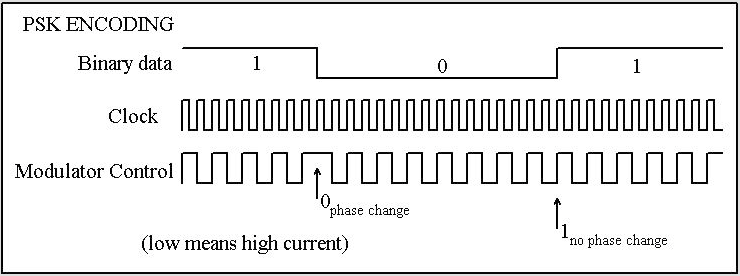
\includegraphics[width=\textwidth]{03_Theory/figures/PSK.png}
    \caption{PSK encoded RFID tag output}
    \label{fig:03:PSK}
\end{figure}

\newpage
\subsubsection{Manchester}
One of the more popular types of ecoding is manchester encoding. It is a variant of biphase where you allways find a levelshift in the middle of each bit. A shift from low to high will yeald a "1" and visa versa. This means that if one has a "1" and a "0" back to back, one will see no change for the equivalent of one bit length. \cite{ManchesterAtmel,forster2000manchester,Manchester}
\begin{figure}[H]
    \centering
    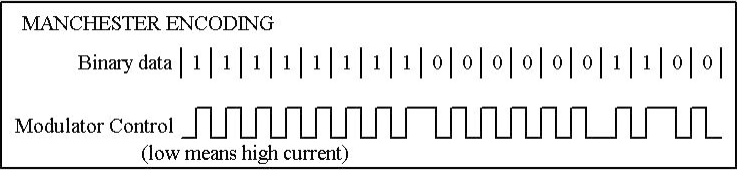
\includegraphics[width=\textwidth]{03_Theory/figures/Manchester.png}
    \caption{Manchester encoded RFID tag output}
    \label{fig:03:Manchester}
\end{figure}

\subsection{T5557}
Microchip Technology Inc. has its own, more complex RFID protocoll, T5557. \cite{T5557priority} The T5557 protocol has a greater capacity at 
\todo{Fill section}

\subsection{Reader distance}
\cite{microID125}
\todo{Fill section}
\subsection{Position detection}
Position detection using RFID can be done in two main ways, triangulation \cite{triangulationbritannica_2011} or area detection. \cite{cho2014rfid} Both have their advantages and disadvantages.\\

With trilateration one needs less antennas as three points of reference is enough to detect position in 2D. While this holds true it is necessary to have some form of active tag to achieve this as the noise ratio likely would be too high in a confined space.\\

Area detection is done by having an antenna per location one wishes to detect a tag. This can be done at the resolution the the application demands. The downside of this is that one needs one antenna for each area one wants to detect tags, and if several tags are within the range of the same antenna, there is no way to determine where they are within the antenna area, so sufficiently small antennas are needed.\\

Mark Roberti, founder and editor at the RFID Journal stated in 2016 that the only feasible way to detect multiple pieces in a small array only using passive tags would be area detection by small coil antennas. \cite{roberti_francois}


\subsection{Anti -collision}

Anti-collision is a feature added to RFID systems where it is desired to detect more than one tag at any given moment. This introduces more complex code and/or hardware. As RFID becomes more prevalent in credit cards and other tags with the same form factor, given a user with multiple RFID tags in its wallet, it would be beneficial if the reader would be able to detect a valid ID even though presented with multiple invalid once at the same time.\\

Software wise one has to filter out the signal of both or more than one tag, which becomes increasingly difficult as more tags are introduced.\\

It is possible with more complex tags to give them a priority ID that will make the tags wait for their turn to transmit. This will as a result make the total read time linearly longer with the introduction of more tags. \\



\section{Frequency}
\subsection{15.36 MHz}
\todo{Fill section}
\subsection{125 kHz}
\todo{Fill section}
Mention the length of one bit





\section{Antenna}
The wavelength of a 125kHz radio wave is the speed of light c devided by 125 000, since the radio waves, like all electromagnetic waves travel at the speed of light.

\begin{align*}
    \text{Wave length} = \frac{299 792 458m}{125000}\approx 2400 m
\end{align*}
A true dipole antenna will hence be a tall order, as each monopole will be 600m long. For this reason, a much more rational approach of using antenna coils that resonates at the wanted frequency are used in low frequency applications such as RFID.\\

The inductance of an antenna coil is highly dependent on its shape, be it round, square, snakelike. Also, it depends on the resistance in the material used, whether it is multilayered or not, thickness of the material used, and an array of other electrical properties. The formulas for the inductance one can expect out of a given coil is therefore quite different for all these different shapes, with constants relating to the previous named variables. \cite{antennadesign} The two types of antennas that are of interest in this 125kHz application are circular and rectangular, both multilayered.\\



From \cite{antennadesign} we find that the equation the inductance of a n-turn rectangular multilayered coil can be formulated as:

\begin{align}
    L=\frac{0.0276 (CN)^2}{1.908C +9b+10h} [\mu H]
\end{align}
where

\begin{align*}
    &\text{N = number of turns}\\
    &\text{C = x+y+2h}\\
    &\text{x = width of coil}\\
    &\text{y = length of coil}\\
    &\text{b = width of cross section}\\
    &\text{h = height of cross section}\\
\end{align*}

\begin{figure}[H]
    \centering
    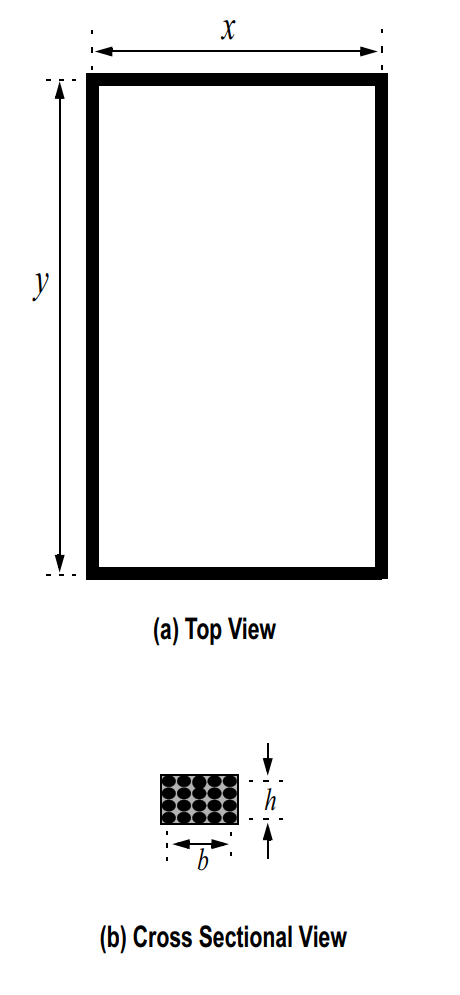
\includegraphics[width=0.5\textwidth]{03_Theory/figures/coilAntenna.png}
    \caption{N-turn square loop coil with multiple layer}
    \label{fig:03:coilantenna}
\end{figure}

\todo{Fill section}

\section{Chess board}
\todo{Fill section}

